\chapter{Spieler}

Das Spieler Objekt enth"alt als Kindobjekte seine Spielfiguren. Als Skripte h"angen ihm eine Player Component, sowie eine Input Component an. 
\section{Player Component}
\begin{lstlisting}[breaklines=true]
GameObject[] figurines = new GameObject[3]; //Alle Figuren ueber die ein Spieler verfuegt
public int actionPoints = 0; //Anzahl an verfuegbaren Aktionspunkten
int maxAP; //Maxcap für AP
\end{lstlisting}
Das Skript speichert die maximale Anzahl an Aktionspunkten, die f"ur die verschiedenen Fraktionen variieren, f"ullt nach dem Ende der Runde die Aktionspunkte beider Fraktionen auf und stellt sicher, dass dabei die Zahl der erhaltenen Aktionspunkte nicht die Grenze "uberschreiten. 

\begin{figure}
	\centering
	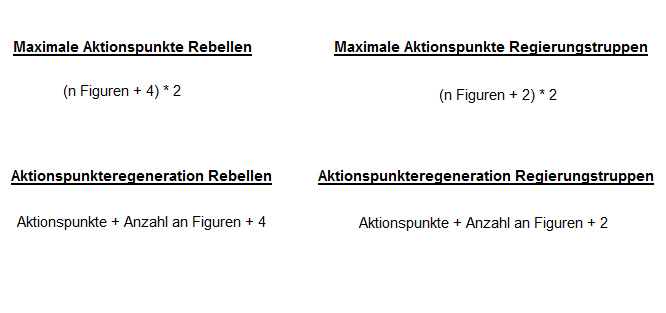
\includegraphics[height=5cm]{images/Aktionspunkte.png}
	\caption{Berechnung der Aktionspunkte}
	\label{fig:Aktionspunkte}
\end{figure}

\section{Input Component}


